\section{Remote Procedure Call}

\subsection{Definition}

\subsection{Motivation}
%  this is just to warmup 
With the emerging technology to the cloud many protocols wanted to take the lead.
Nowdays most of the architectures are based on multi-servicces and micro services.
And to have higher versatility of developpers mulptile companies choose to be open to different programming langauges. basically it would be more efficient if we take advantage of each programming language to satisfy a specific need.
However the callenge nowdays is to make the bridge between those plateforms.
We have many initiatives such as openapi that try to create a taxonomy for rest apis.
other approachs is to impelement all the different interfaces of the protocol by them selfs such as the RPC
\subsection{State of the art}

\subsection{Research Questions}
In this section we will first explore the ease of implemenation of this protocol
then we will try to answer the following Research questions

\begin{description}
    \item[\textsc{RQ}~1:] How do RPC implementations react to the size of the request ?
    \item[\textsc{RQ}~2:] How do RPC implementations react to the number of clients ?

\end{description}
\subsection{Experimental protocol}
\subsubsection{Hardware settings}
All the experiments are run on the cluster paravance of the G5K platform. This cluster is composed of 72 identical machines, each one is equipped with 2 Intel Xeon E5-2630 V3, with 128 GIB of RAM. For more accuracy, our SUT (System Under Test) is equipped with a minimal version of Debian 9 (4.9.0 kernel version), which enforces the core processes required for the purpose of our experiment. Furthermore, we used Docker containers technology for reproducibility of the experiments and the isolation of the servers.
\subsubsection{Energy measurements}
To report on the energy consumption, we used HWPC sensor [], which is based on Intel RAPL technology, one of the most accurate tools to measure the energy consumption of the CPU and DRAM []. For better accuracy, we ran the HPWC sensor with a frequency of 10 Hz, and we used the same machine for all the experiments in order to reduce the variability [].

\begin{figure}[!hbt]
    \begin{center}
        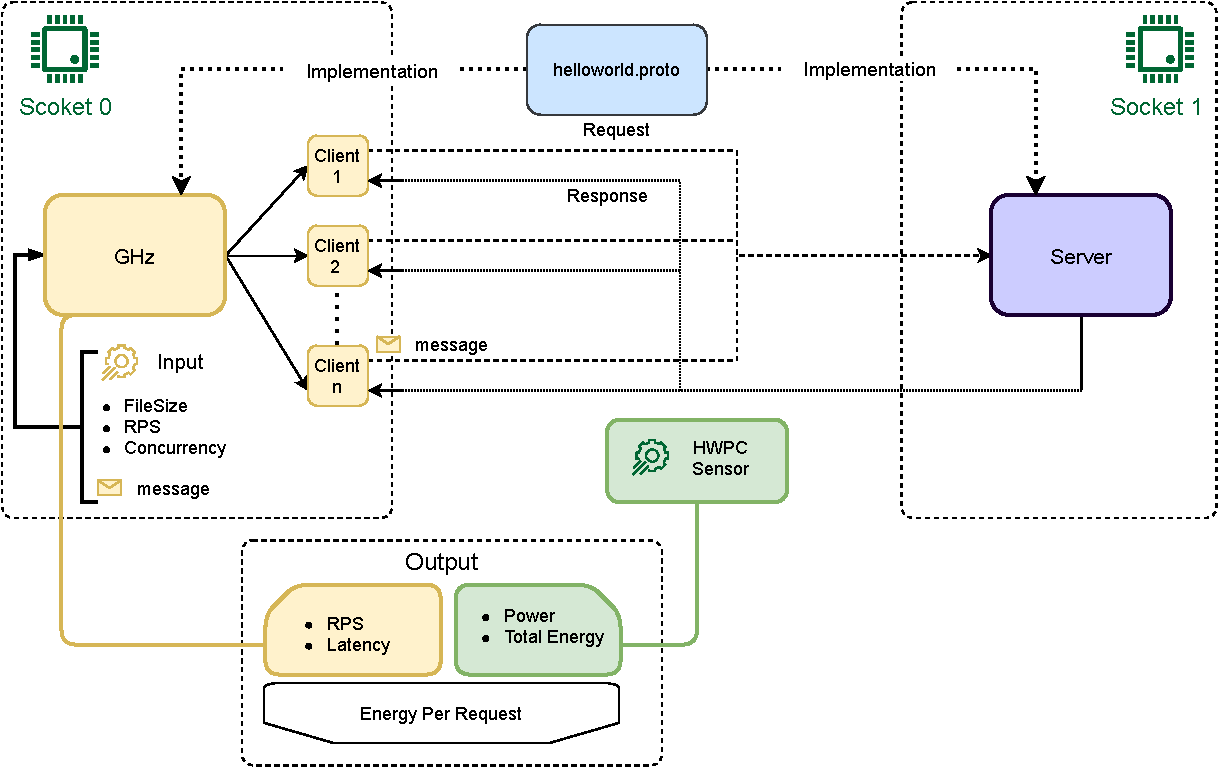
\includegraphics[width=.8\linewidth]{imgs/rpcprotocol}
    \end{center}
    \caption{Experemenal software architecture}\label{fig:rpcprotocol}
\end{figure}
\subsubsection{Client and server environments}

To limit the impact of the network on the experiments, we run both the client and the server on the same machine. However, we isolate each one on a different socket, in order to reduce the effect that the client might have on the server ones and vise-versa. To do so, for each iteration, we always run the same client on Socket 0 and the server that we want to test on socket 1. Both the server and the client take the whole socket for their experiment. In addition all the extra services, such as OS, hwpc, etc. are run on Socket 0. Therefore, the only process being executed in Socket 1 is the server that we benchmark.

\paragraph{Client :}
% TODO : add the github repository links 
For better accuracy and more details, We use an updated version of the open source RPC benchmarking tool, named GHZ (https://ghz.sh/).
The modified version allows us to get the average power for each request form both the server and the client sides.
The new version is available in the repo.
The client will take the protocol description to generate an implementation for the message helloworld, and then fork 50 instances that will send the same request to the server simultaneously.
\paragraph{Server :}
The server implementations are based on the official implementation by Google for most of the languages . Each server uses 16 cores  and is limited to 512 MB of RAM

\subsection{Results and finding}
[\textsc{RQ}~1:] How do RPC implementations react to the size of the data ?
The purpose of this question is to study the behaviour of the server for transferring large objects. To do so, we send to the server 80,000 requests with a size scaling from 10 bytes up to 10 Megabytes, which gives 10,000 requests per size per server. To eliminate extra factors, we let the server handle the rate at which it can answer each request. However, we put a 20 sec timeout limit for each request. Therefore, our boundary condition is only the number of requests received by the server.  For this experiment, we investigate 4 observable variables :
\begin{enumerate}
    \item The average power consumption during the the process : this will indicate the overall behaviour of the server in working mode for long durations ;
    \item The tail latency for the 99th percentile : which indicates how performant is the server ;
    \item The average number of requests per second : which indicates the  average number of clients that  the server can handle ;
    \item The average energy cost of a single request : unlike the first indicator, this one shows how green is the implementation taking performance into consideration.
\end{enumerate}



% TODO : ADD the figures 
The above figure depicts the overall behaviour of each framework based on the size of request (Payload). For each framework, we can distinguish three modes, and they all depend on the payload :
\begin{enumerate}
    \item Stress free mode: when the server has enough resources to satisfy the requests because they require a memory less than a certain threshold (depends on the language and the platform),
    \item Escalation mode: where the requests tend to be bigger, however the server can still manage to handle them, and here where we can see a change in the energetic and performance behaviour.
    \item Broken state mode: when the requests are much heavier and the server break—like 10 MB.
\end{enumerate}

\subsubsection{Stress free mode}
In this mode, the compiled languages tend to consume less resources (av power). JVM-based languages tend to consume more energy, especially Scala. However, we do not observe the same behaviour when it comes to efficiency. Unlike the other interpreted programming languages, PHP performances could be compared to the compiled ones, such as CPP or GO, and even better to some others, such as Swift. JVM-based languages tend to have better performances than the interpreted ones. Furthermore, OpenJDK has shown more efficiency than GraalVM []. Overall, we can have 3 groups when it comes the cost of each request:
\begin{itemize}
    \item Green languages: CPP, GO, RUST, ELIXIR, and PHP
    \item Middle class: Most of the interpreted languages and vm-based ones
    \item Energivore class: Crystal and Scala
\end{itemize}

\subsubsection{Escalation mode}
In this mode, the behaviour of the server depends on the payload. We observe three behaviours
\begin{enumerate}
    \item Drop in performances without an increased power, such as .Net core, Java micronaut, Crystal, and Dart. In this case the server keeps using the same ressources, and sometimes less, because it takes more time to handle the less requests. This class of languages tend to be the most energivore when it comes to the cost per request ;
    \item Increase in power without affecting the performances: such as Go, .Net. The energy consumption of a single request, is affected slightly but still increase ;
    \item Increase in power and drop in performances: Despite the increase of the power consumption, the server becomes slightly slower, which increases the cost of the energy cost per request. This cost is still better than the first case, which concludes  that the servers in the first category are on the verge of breaking.
\end{enumerate}

Special mention to Elixir that kept scaling despite the lack of performances compared  to other compiled languages (Go, CPP)

\subsubsection{Broken state mode }
Only four of the 25 configurations could parse the 10 MB files. And only 1 from those could achieve a 76\% acceptance rate which is Elixir, the other 3 had less than 3\% success rate (Rust, Swift and Dart).
The rest could be divided into two categories:
\begin{itemize}
    \item Timeout : where requests took too much time that the client canceled them, in this category we find most of dynamic codes such as: openJDK, Kotlin ;
    \item The size of request exceeded the maximum size by implementation : this is where the implementation could not handle requests with large size, such as .Net, Go, .Net core, CPP, PHP, Scala, Nodejs, Ruby, Python.
\end{itemize}


[\textsc{RQ}~2:] How do RPC implementations react to the number of clients ?

\subsubsection{Power behaviour}
based on the heatmap, we can distinguish two main modes.
\begin{itemize}
    \item Low number of clients : where the total number of simultaneous clients is less than 100
    \item Moderate to high number of clients : the number of clients exceeds 100
\end{itemize}


\paragraph{Lite mode}
The implementations can be grouped into two main categories :
\begin{enumerate}
    \item Green Frameworks: most of the framework's power consumption is around 33 Watts.
    \item Energivore frameworks : where the average power consumption is higher than 37 Watts.
\end{enumerate}

In each programming category we observe both behaviours green and energivore. Therefore, we conclude that it depends more on the implementation of the library itself rather than the category of the programming language. Scala and Kotlin are an excellent example to support this hypothesis since both of them run on the same virtual machine as Java (openjdk 16.1).Yet, their average power is 130\% higher than the Java implementation .

\paragraph{Stressed mode}
Although the same classes remained the same , Not all the languages had the same evolution. and here we can clearly see that it is correlated with the category of the programming language rather than the implementation itself.\\
We can clearly highlight that after VM based languages have a significant increase in the average power consumption after they receive more than 100 simultaneous clients. This increase reaches almost double.
Except PHP, all the interpreted languages preserved their energetic behaviour. Same for the compiled ones.
Our Hypothesis points to the JIT, since it will compile the code and make it run faster so it will stress the CPU more.\\
A Remarquable behaviour has been noticed for the grallVM, is the decrease of the energy consumption when we increase the number of the clients. This is related to the drop of the performances which was probably due to the bottleneck situation where the GraalVM couldn't handle more than 100 clients simultaneously.

\subsubsection{Performance Behaviour}
In this section we study only the number of requests per seconds processed by the server without looking at its energy.
We have three observable variables
\begin{itemize}
    \item Satisfaction ratio : how many requerts have been satisfied among the total requests
    \item Request Per Seconds : The number of the requests that have been answered from the server
    \item TailLatency at 99\% : one of the best metrics to evaluate the performances of a server
\end{itemize}

\paragraph{Satisfaction ratio}
Most of the frameworks tried to satisfy all the requests, by either reducing the number of requests per second or by increasing the time of the treatment. However, there are some frameworks that have chosen a different approach such as dart or scalla where the choice was to keep a certain limit of latency even if not all the requests are answered.\\
Furthermore, we tend to see this behaviour among other frameworks such as Python or Asynchronous NodeJs when the number of the client exceeds 800.
\paragraph{RPS}
Most of the servers hit their RPS limit after 5 clients and 100 clients for vm based servers, and after this the number keeps constant. which will decrease the average RPS per client.\\
.net Server is the most performant one, and after him we see JAVA and Go in second place, on the other end Python and ruby are the least performant.
\paragraph{Tail LAtency}
However, the increase in the number of requests per second, doesn't necessarily mean a lower Latency.
As we see in the table ... until the 1000 clients, Go provides the least Latency beside .net.\\
GraalVM provides the highest latency, on average. However, dart tends to become slower when we increase the number of clients, until we pass the 600 simultaneous clients, and there it changes its behaviour, instead of satisfying most the requests it notify the clients directly that the server is saturated, hence a drop in satisfaction ratio, and an amelioration for the Average Latency.


\subsubsection{Energy Per Request}
Now after we made a separation between The energy and The performances, we have seen that most of the performance servers tend to be energy hungry, so we propose to investigate this trade off between the energy and the performance. Todo so we will give an average cost of a single Request in Joules.
Except GraalVM when the cost of the a single request increases with when we add more clients, All the frameworks keep a constant cost,
Java, .net and go are the greenest. and Python, ruby are the most costly with 10x higher.
Therefore we conclude that the number of clients won't impact the energy that much.
Next study will be the payload and how the size of the requests will affect the energy consumption of the framework

\begin{figure}[!hbt]
    \begin{center}
        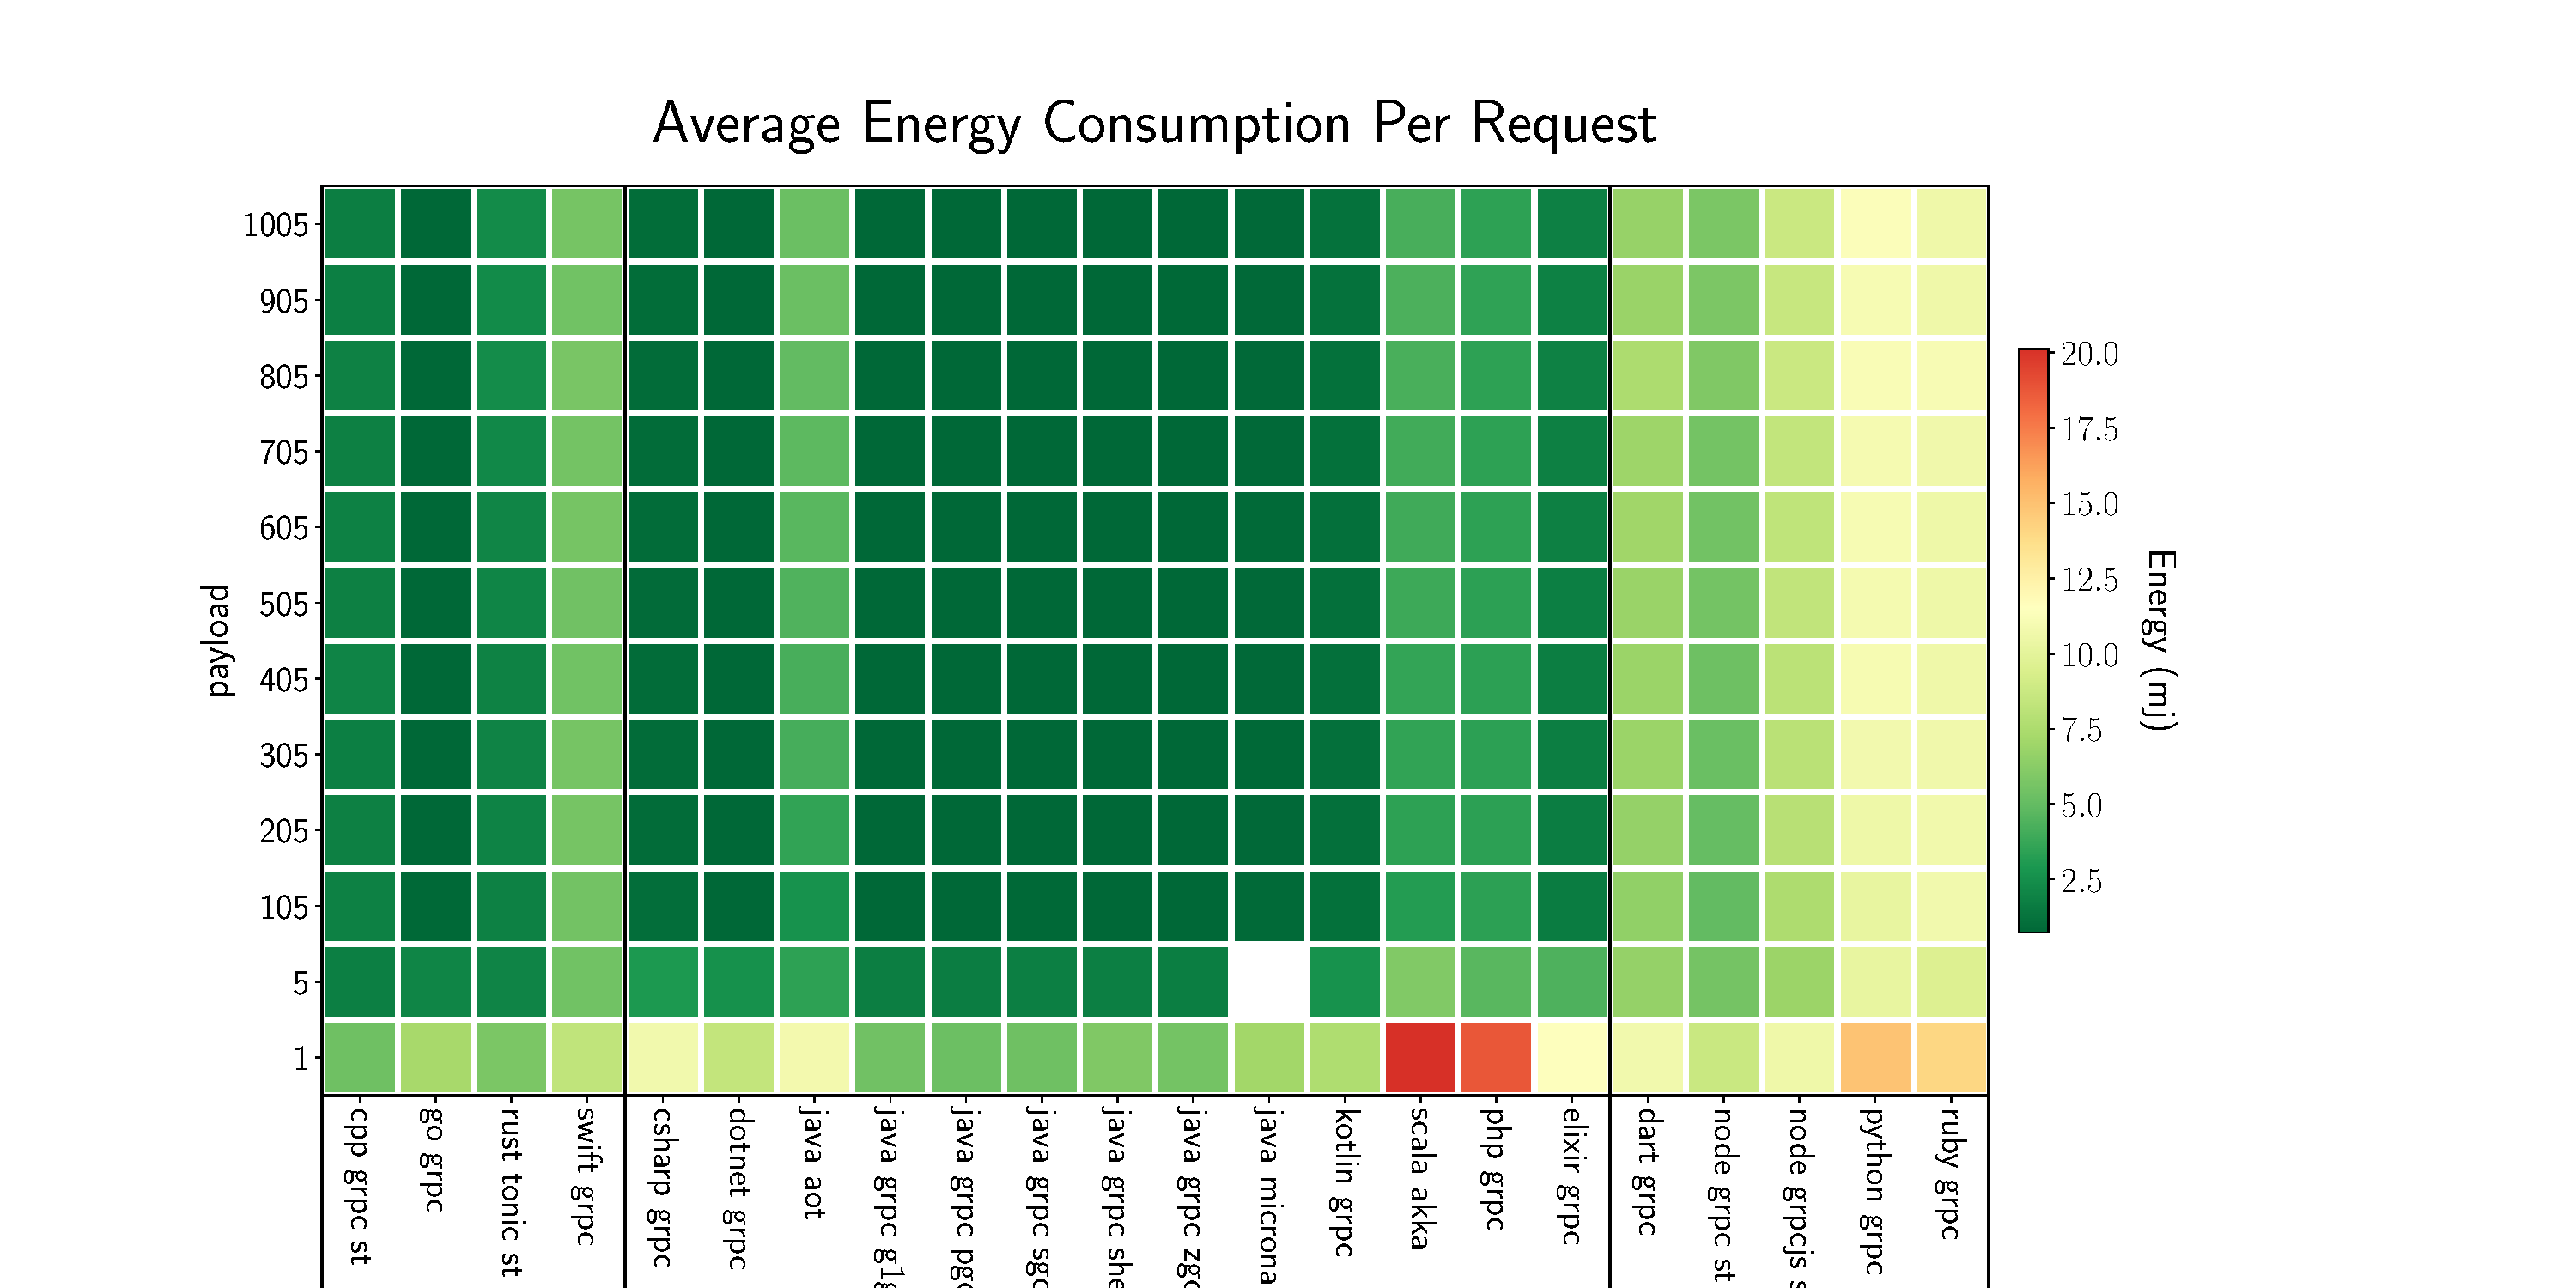
\includegraphics[width=1.2\linewidth]{imgs/rpc_images/energy_cost_clients}
    \end{center}
    \caption{Experemenal software architecture}\label{fig:rpcprotocol}
\end{figure}

\begin{figure}[!hbt]
    \begin{center}
        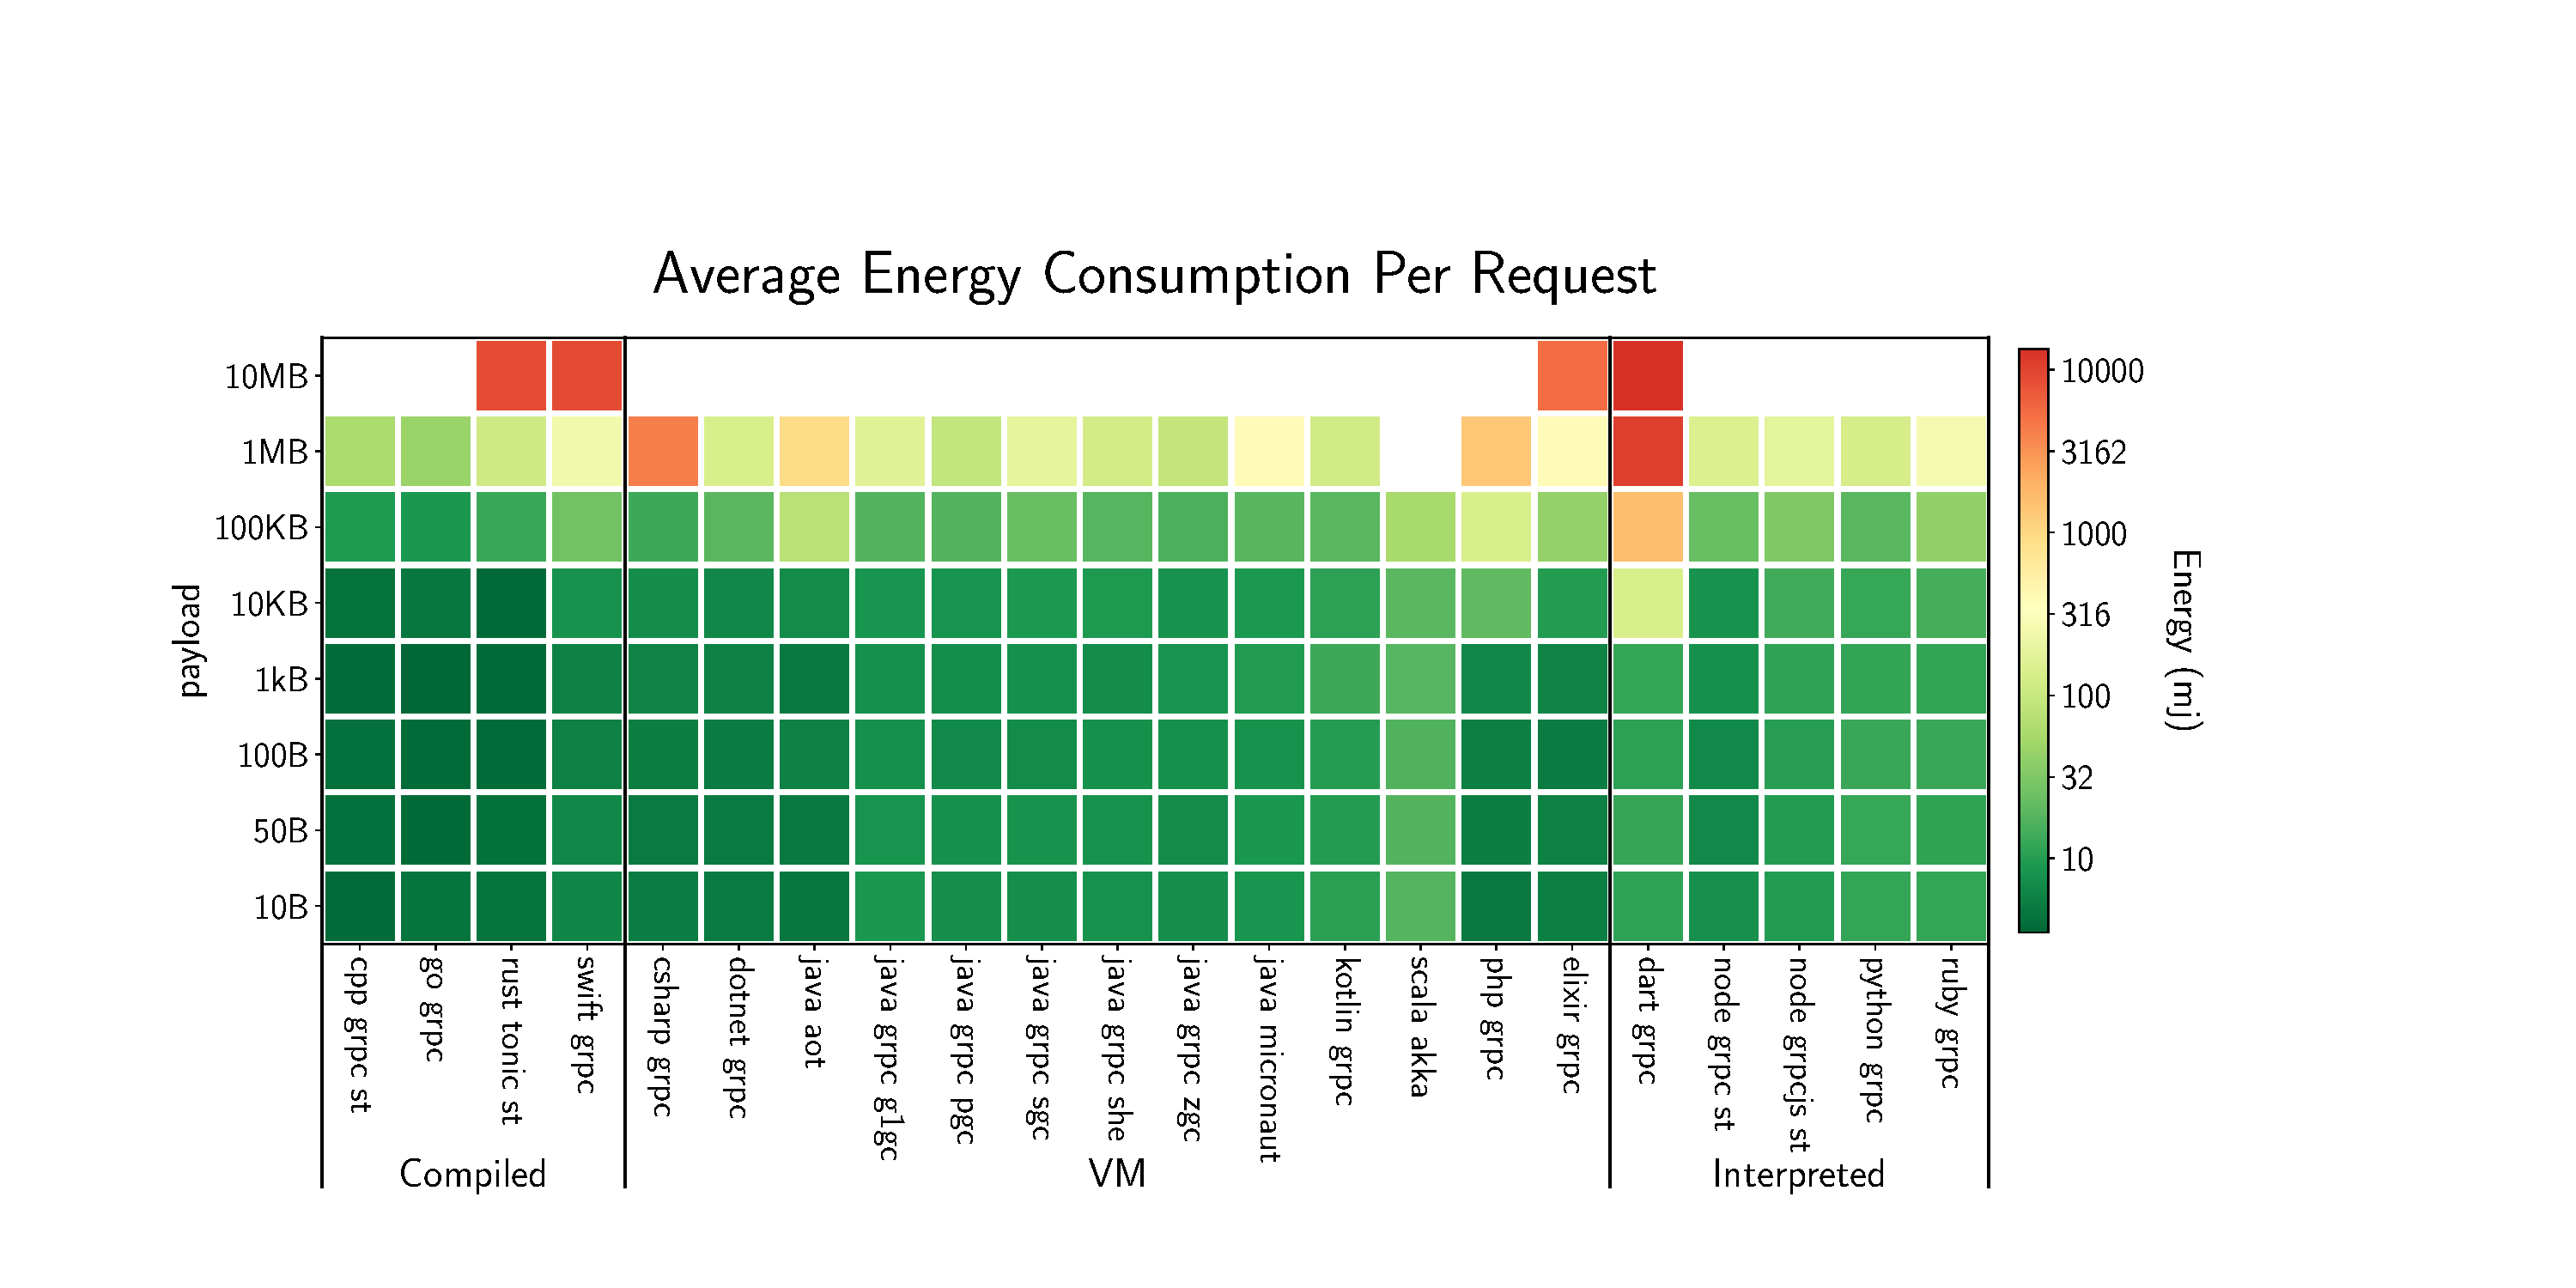
\includegraphics[width=1.2\linewidth]{imgs/rpc_images/energy_cost_payload}
    \end{center}
    \caption{Experemenal software architecture}\label{fig:energy_cost_payload}
\end{figure}

\begin{figure}[!hbt]
    \begin{center}
        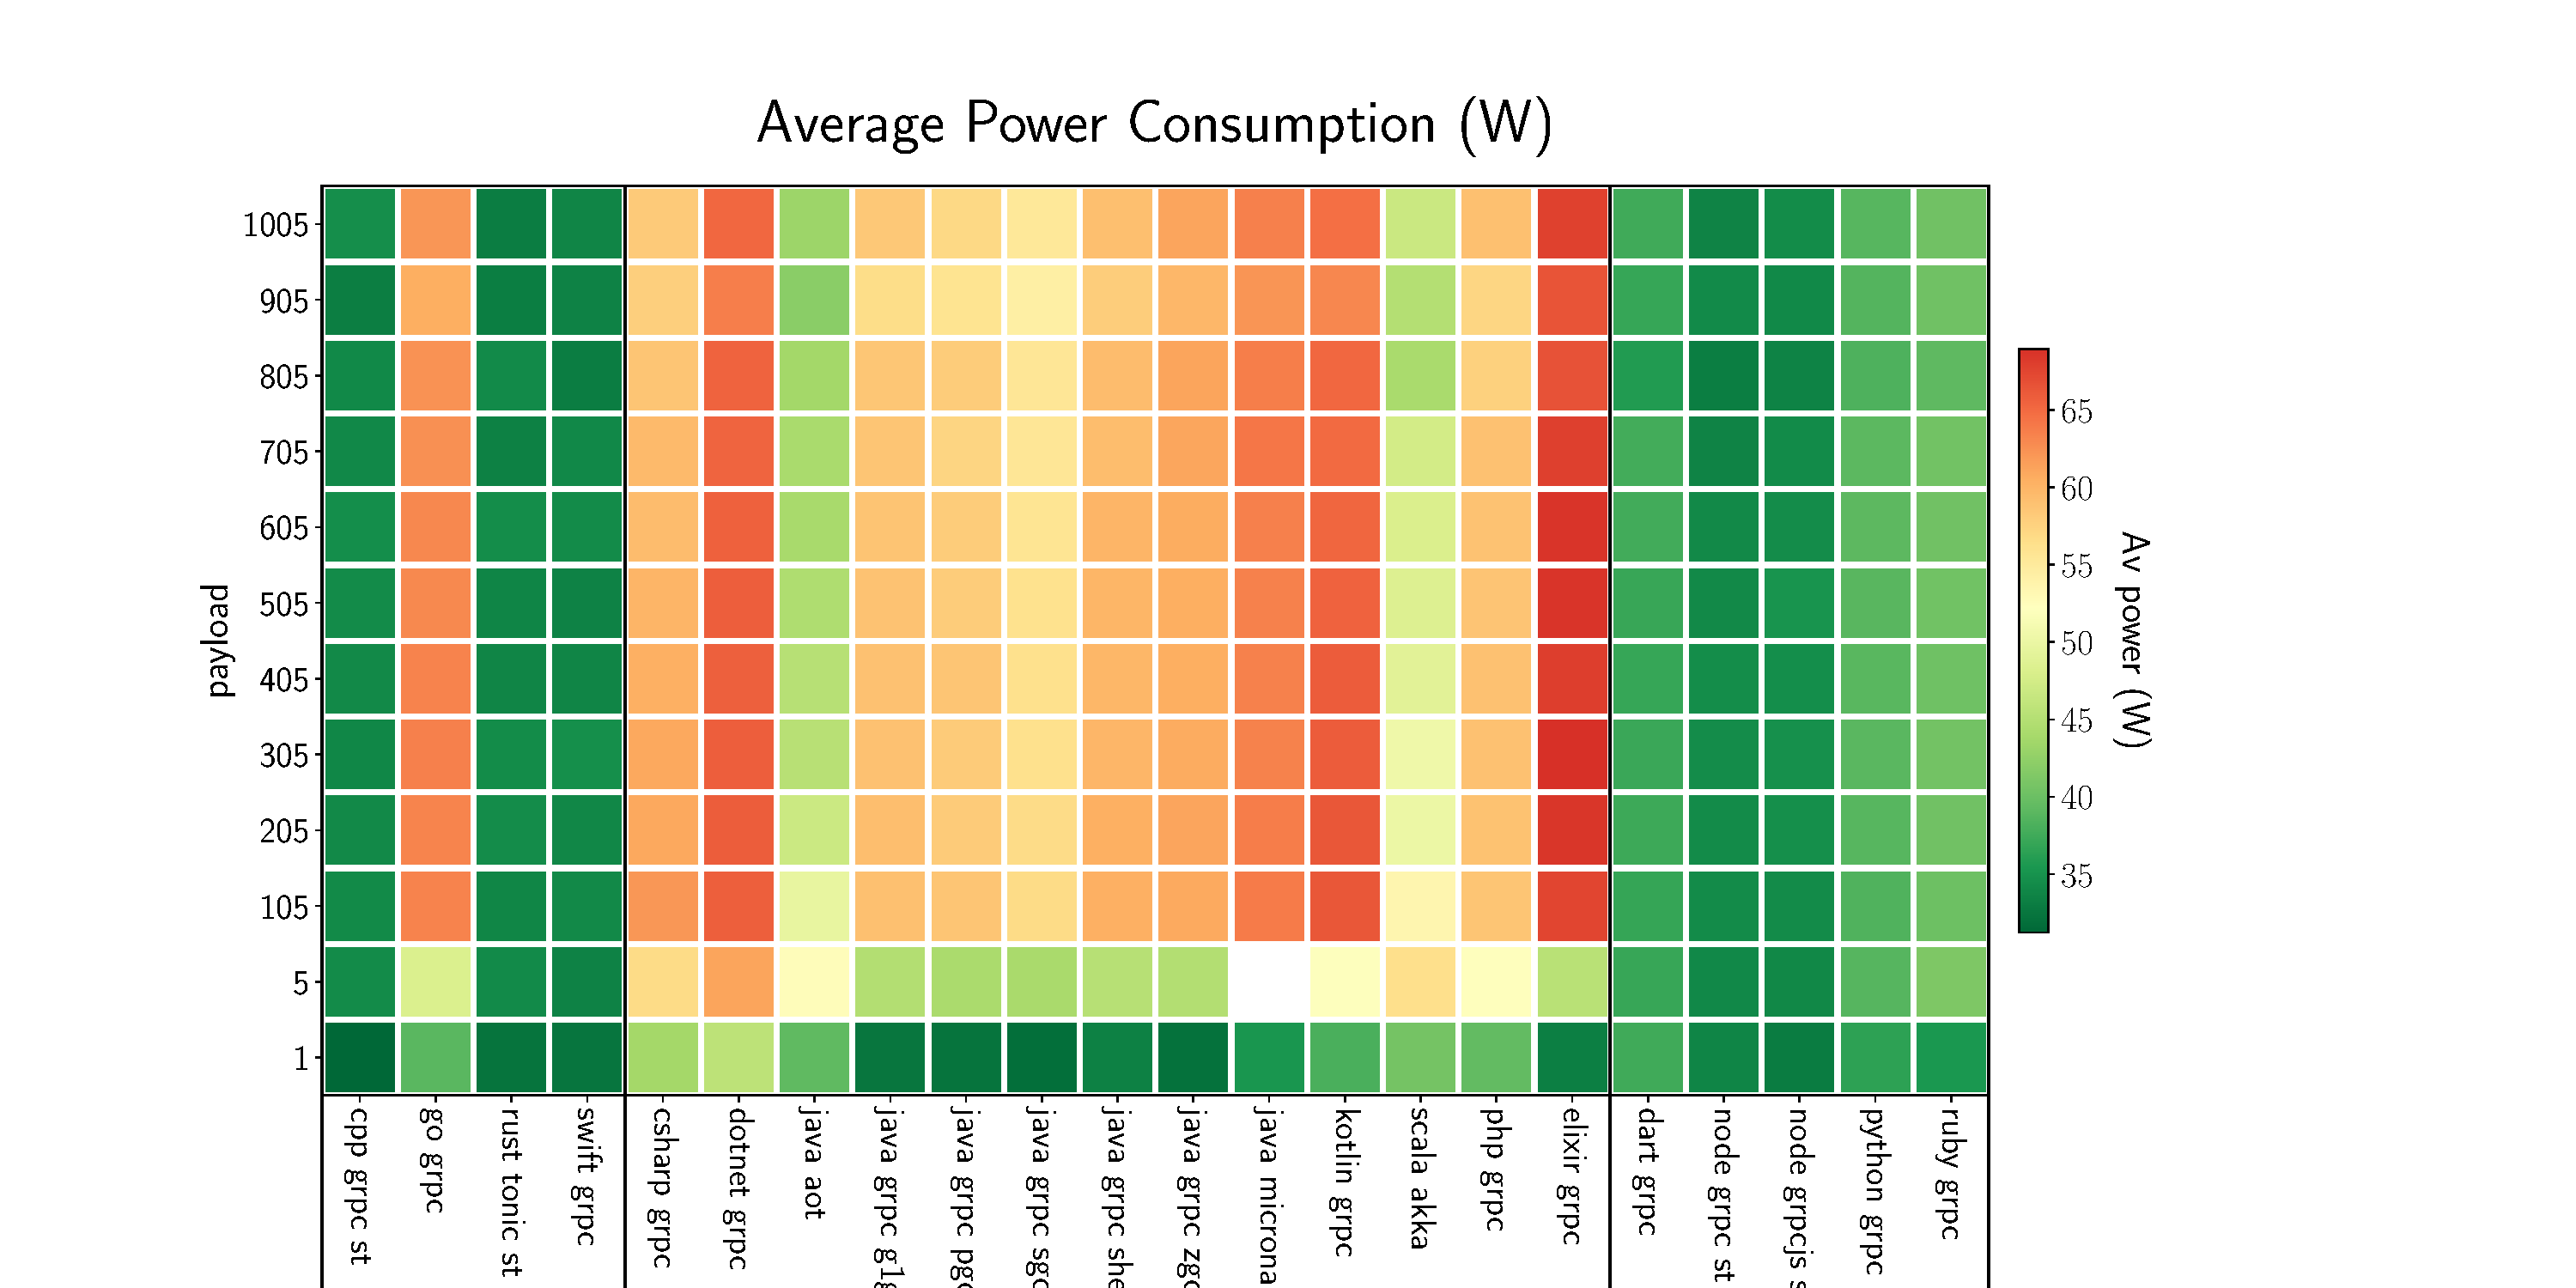
\includegraphics[width=1.2\linewidth]{imgs/rpc_images/power_consumption_clients}
    \end{center}
    \caption{Experemenal software architecture}\label{fig:power_consumption_clients}
\end{figure}


\begin{figure}[!hbt]
    \begin{center}
        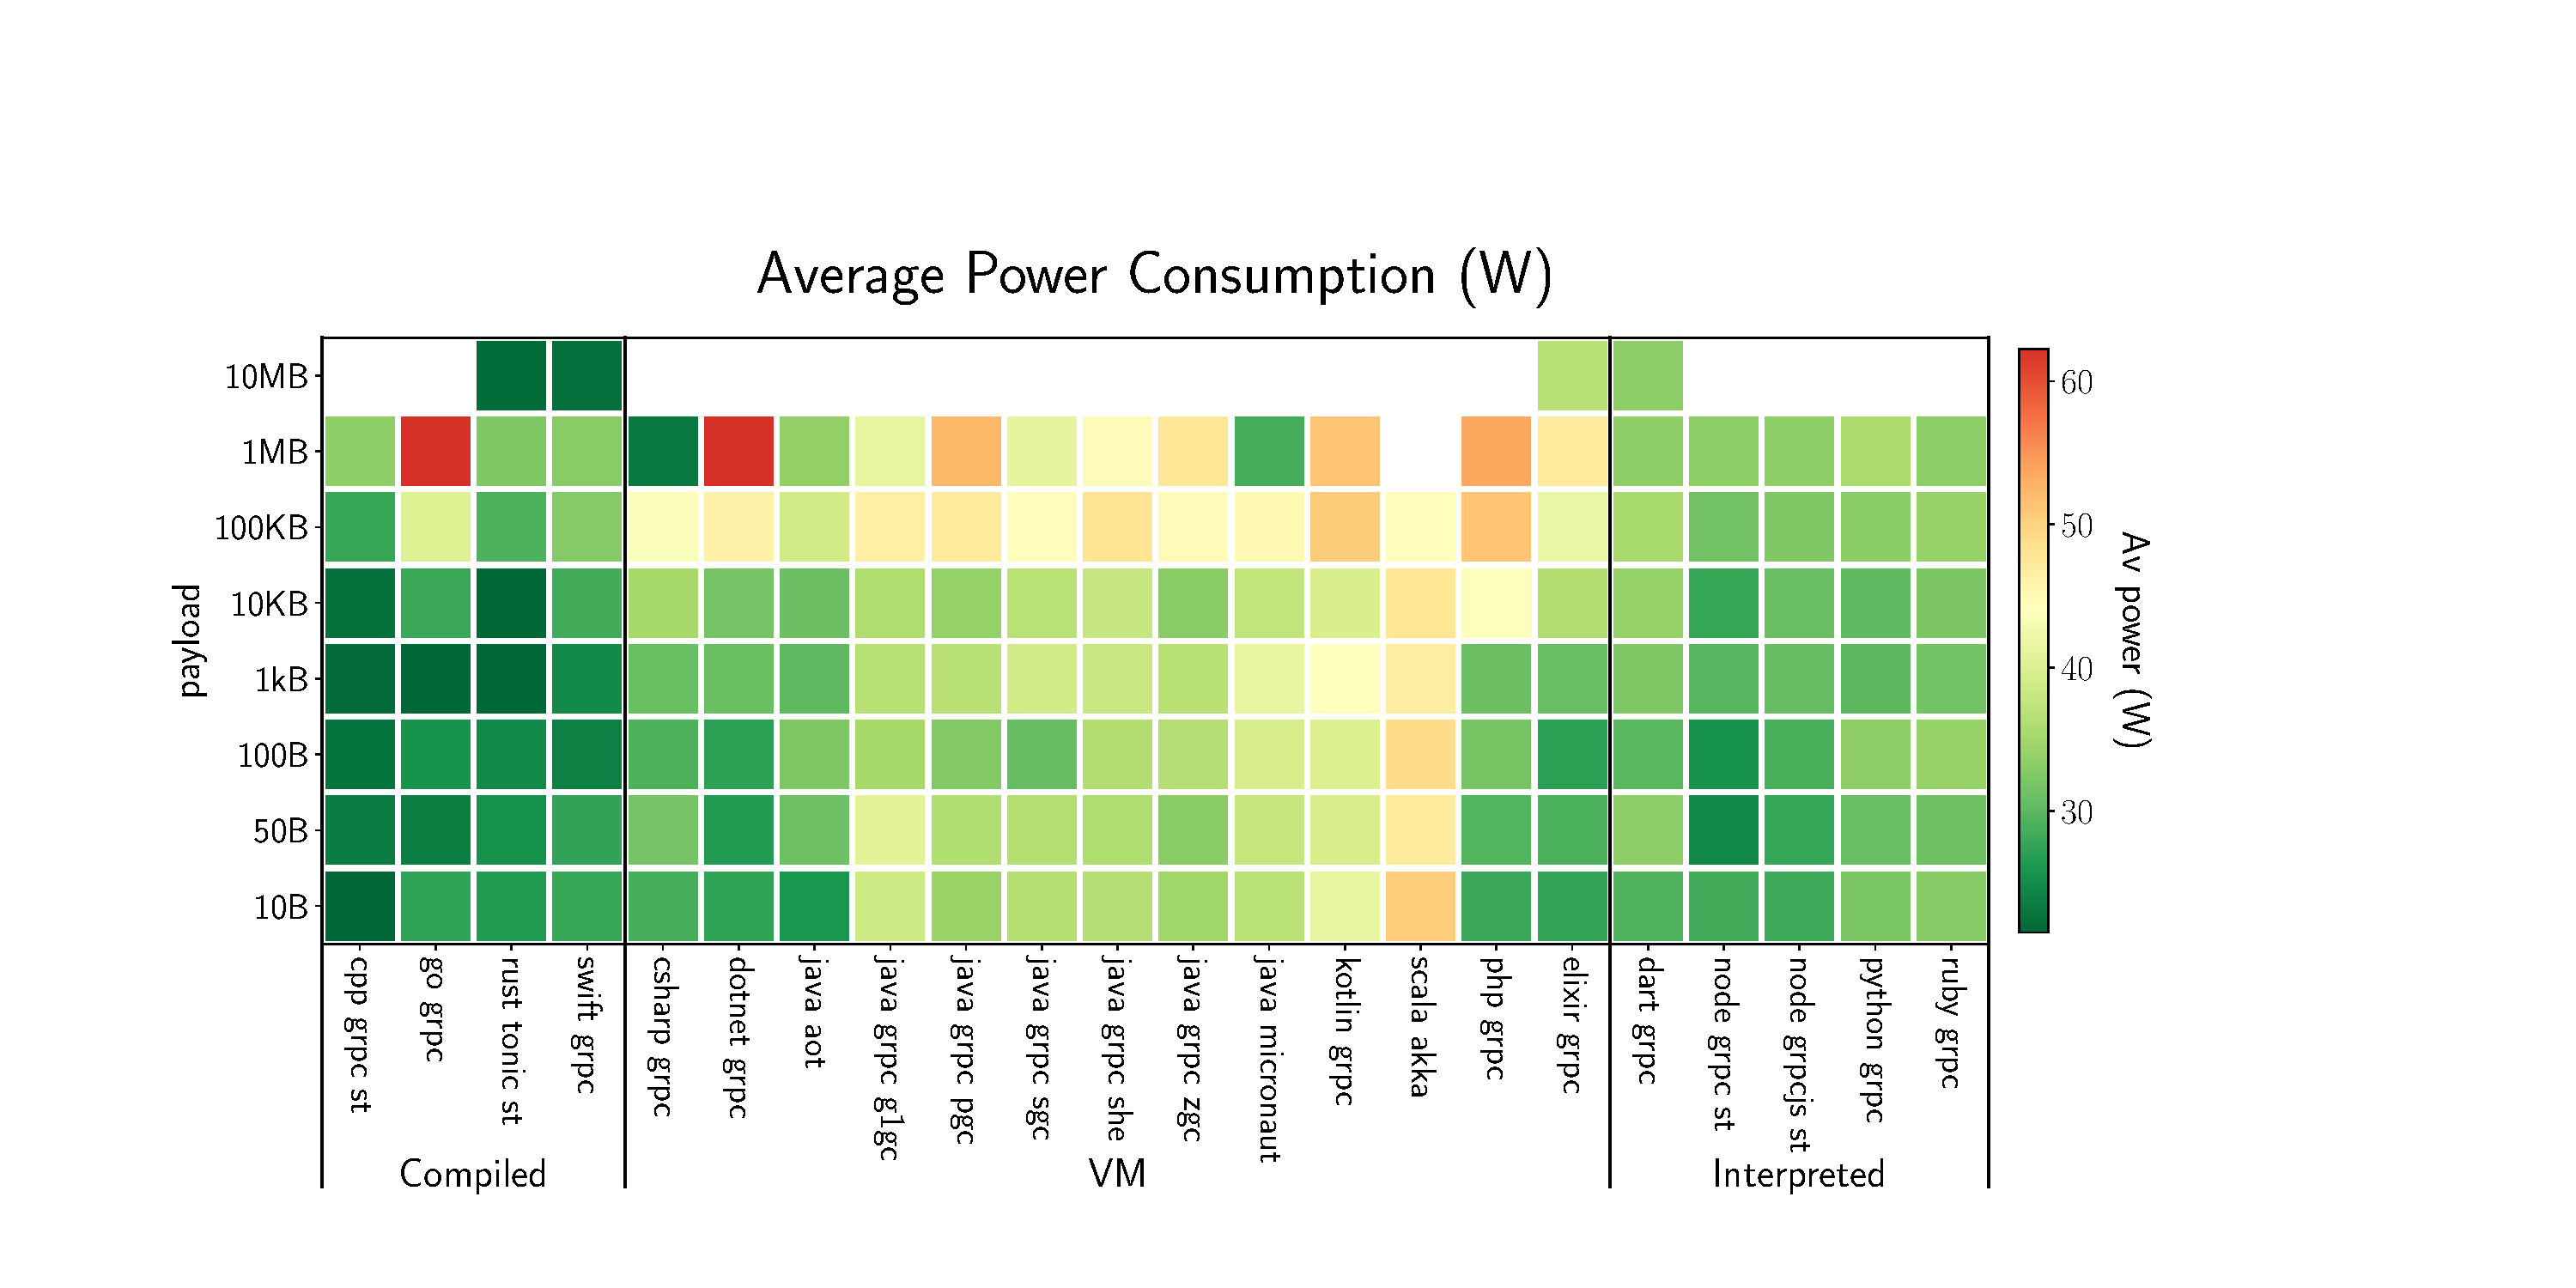
\includegraphics[width=1.2\linewidth]{imgs/rpc_images/power_consumption_payload}
    \end{center}
    \caption{Experemenal software architecture}\label{fig:power_consumption_payload}
\end{figure}

\begin{figure}[!hbt]
    \begin{center}
        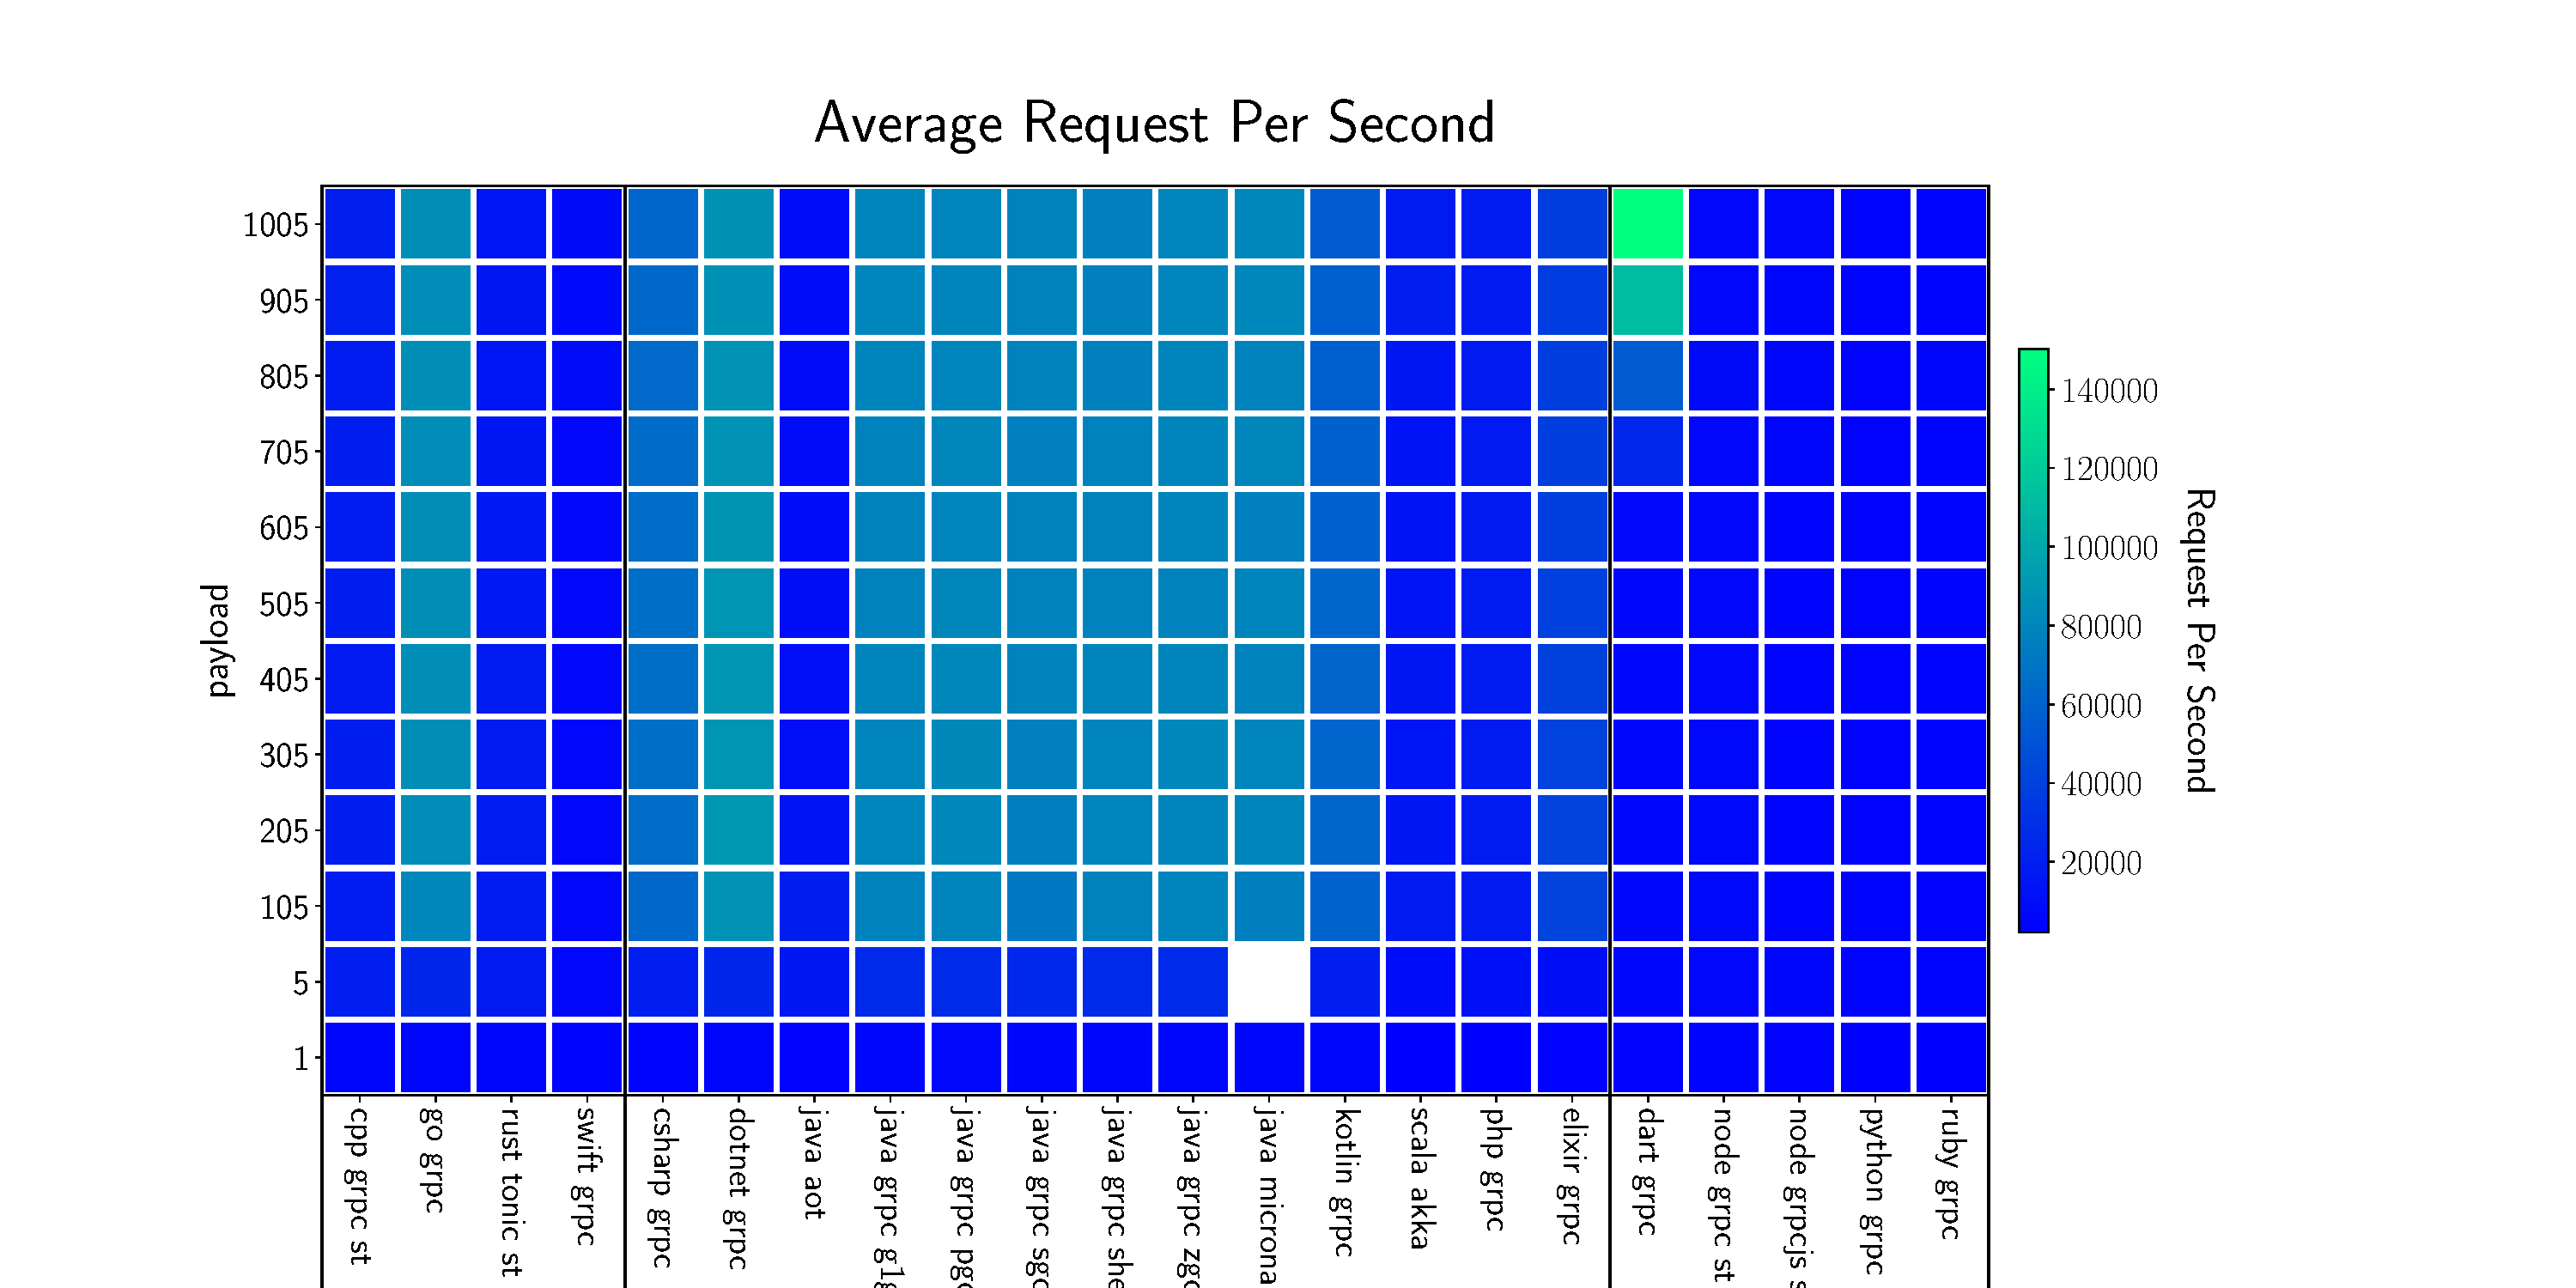
\includegraphics[width=1.2\linewidth]{imgs/rpc_images/rps_clients}
    \end{center}
    \caption{Experemenal software architecture}\label{fig:rps_clients}
\end{figure}

\begin{figure}[!hbt]
    \begin{center}
        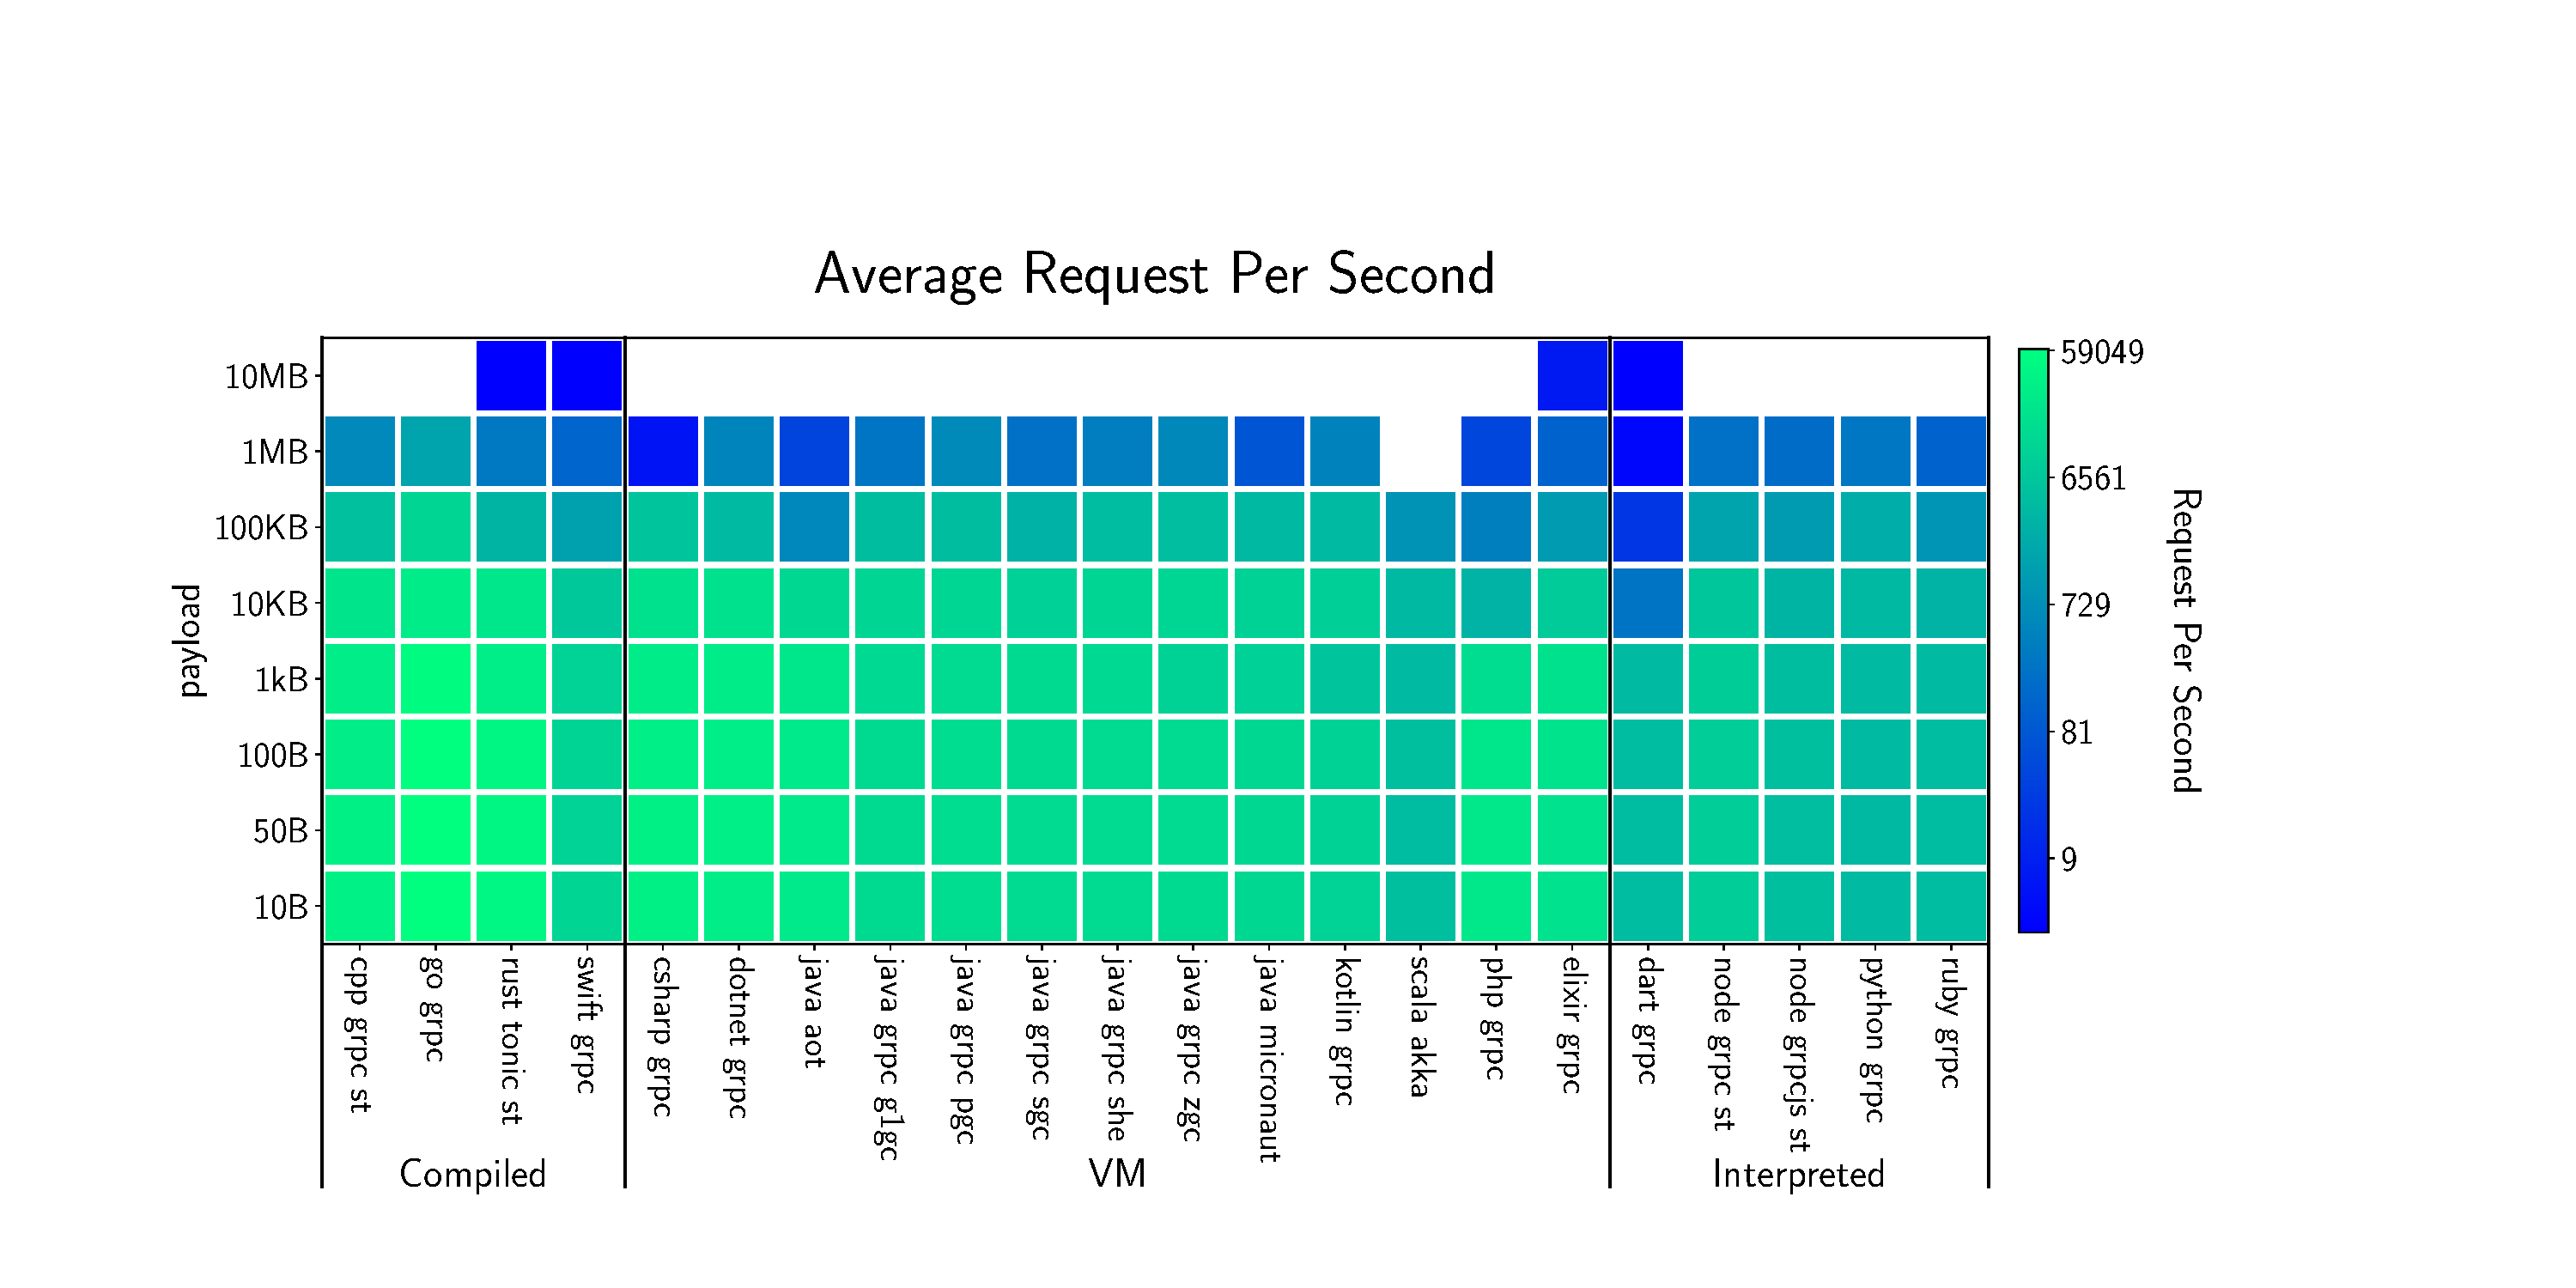
\includegraphics[width=1.2\linewidth]{imgs/rpc_images/rps_payload}
    \end{center}
    \caption{Experemenal software architecture}\label{fig:rps_payload}
\end{figure}



\begin{figure}[!hbt]
    \begin{center}
        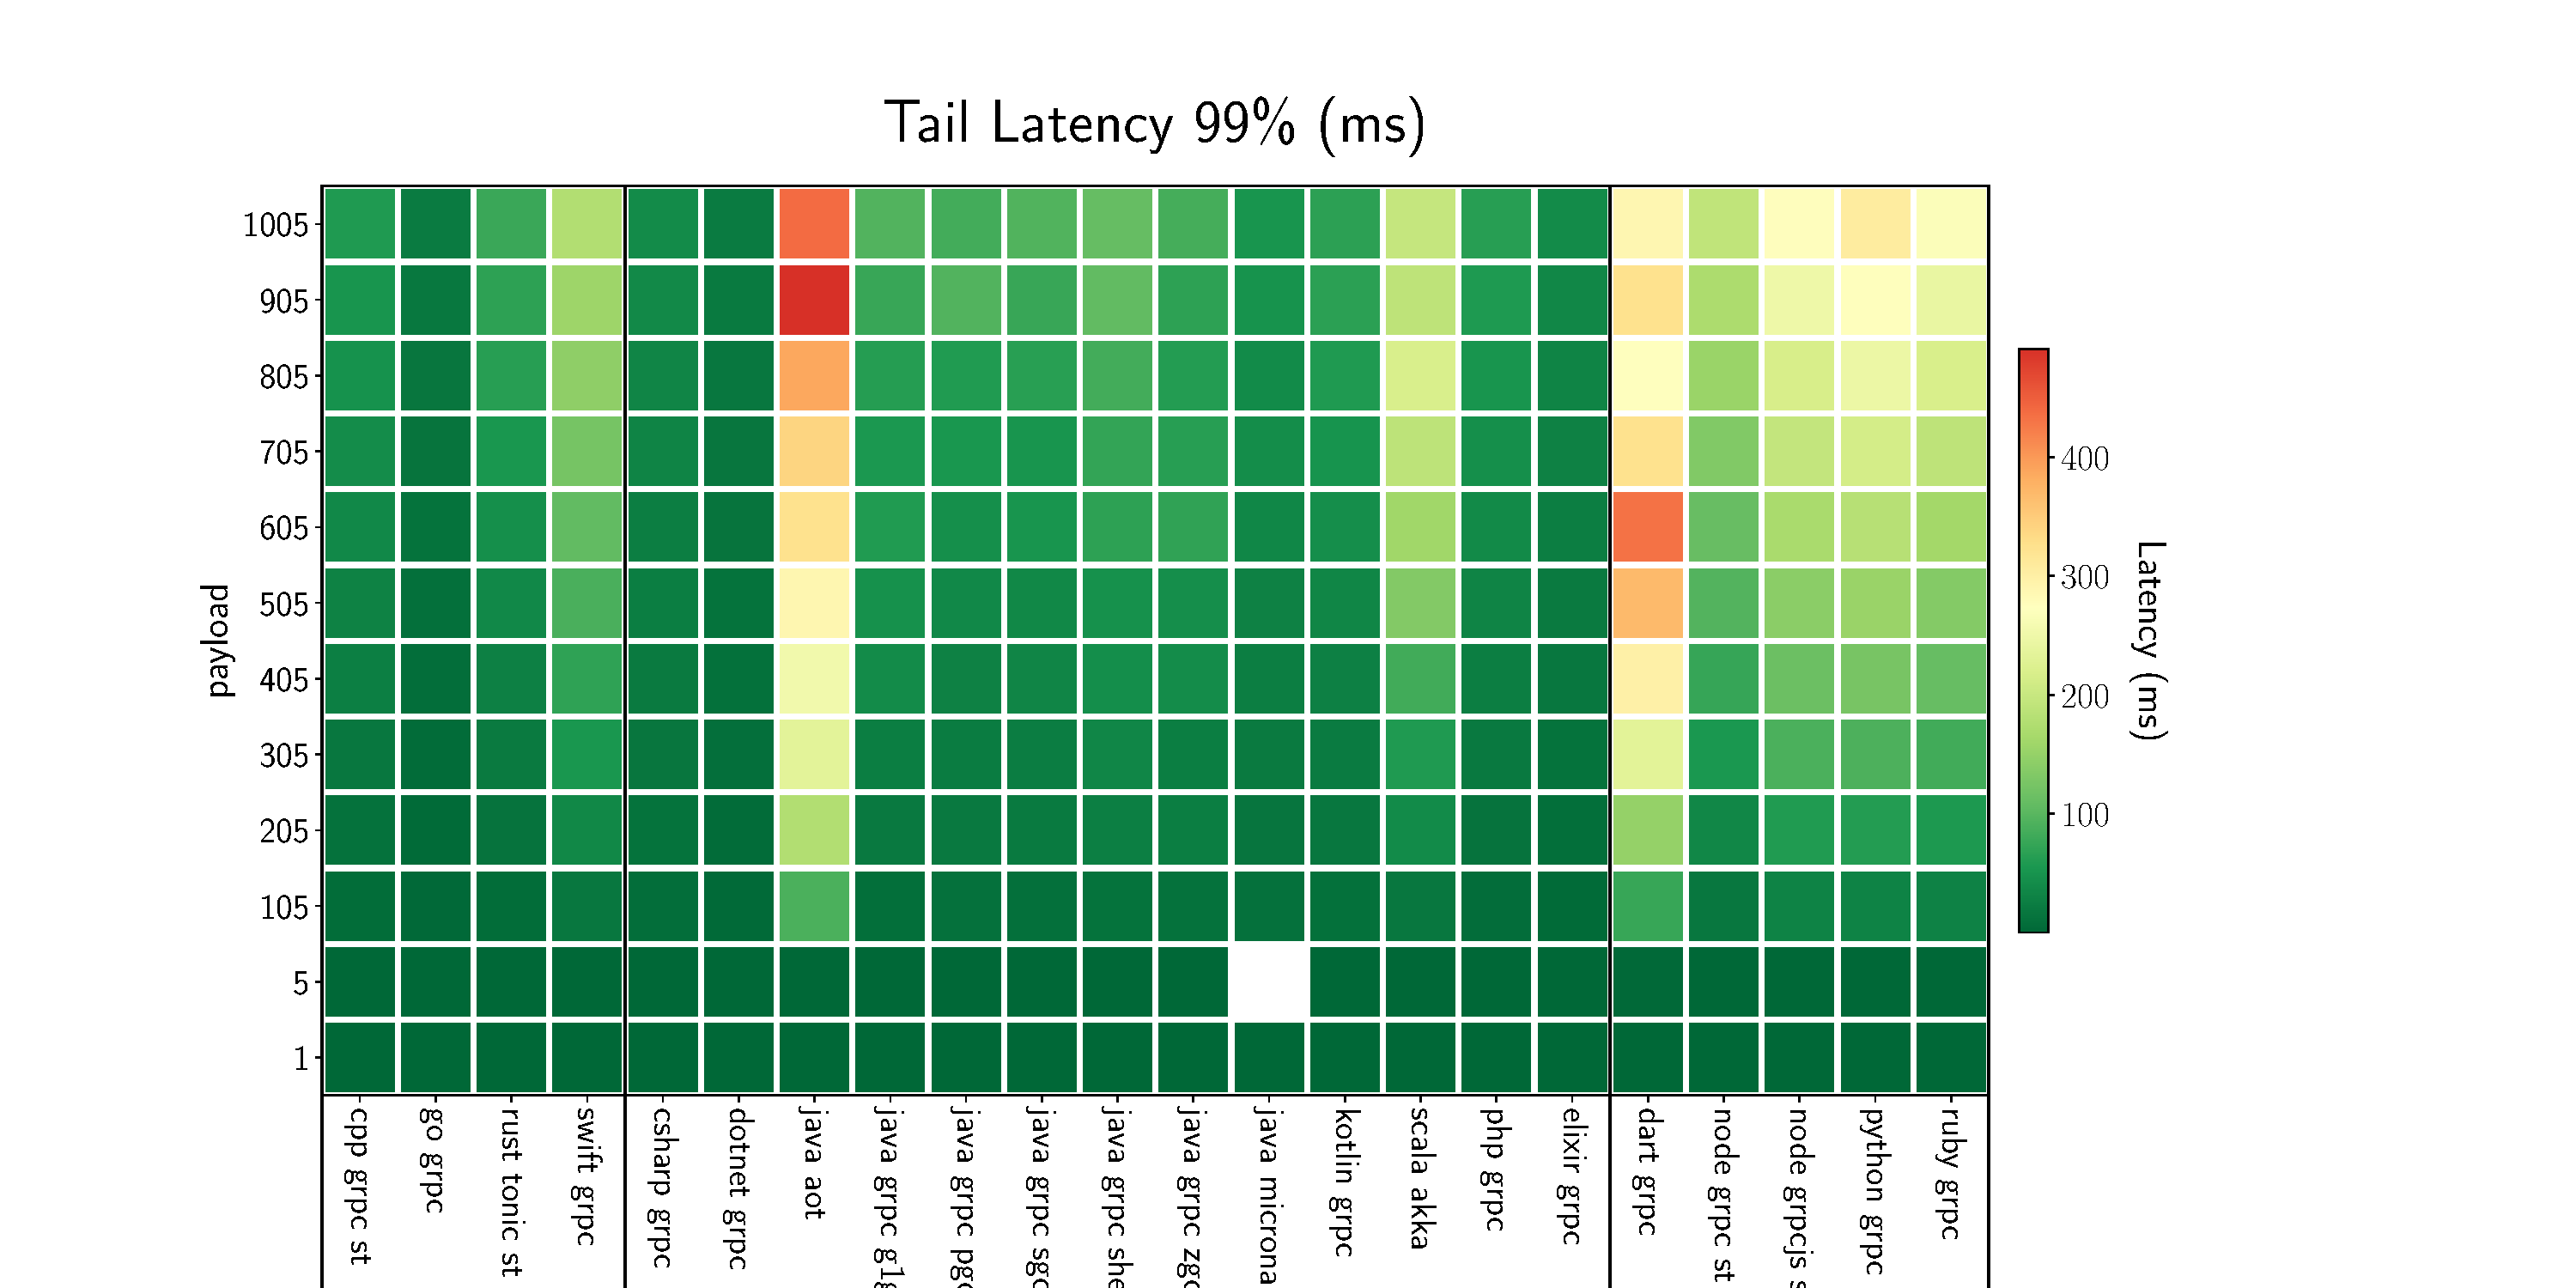
\includegraphics[width=1.2\linewidth]{imgs/rpc_images/tail99_clients}
    \end{center}
    \caption{Experemenal software architecture}\label{fig:tail99_clients}
\end{figure}


\begin{figure}[!hbt]
    \begin{center}
        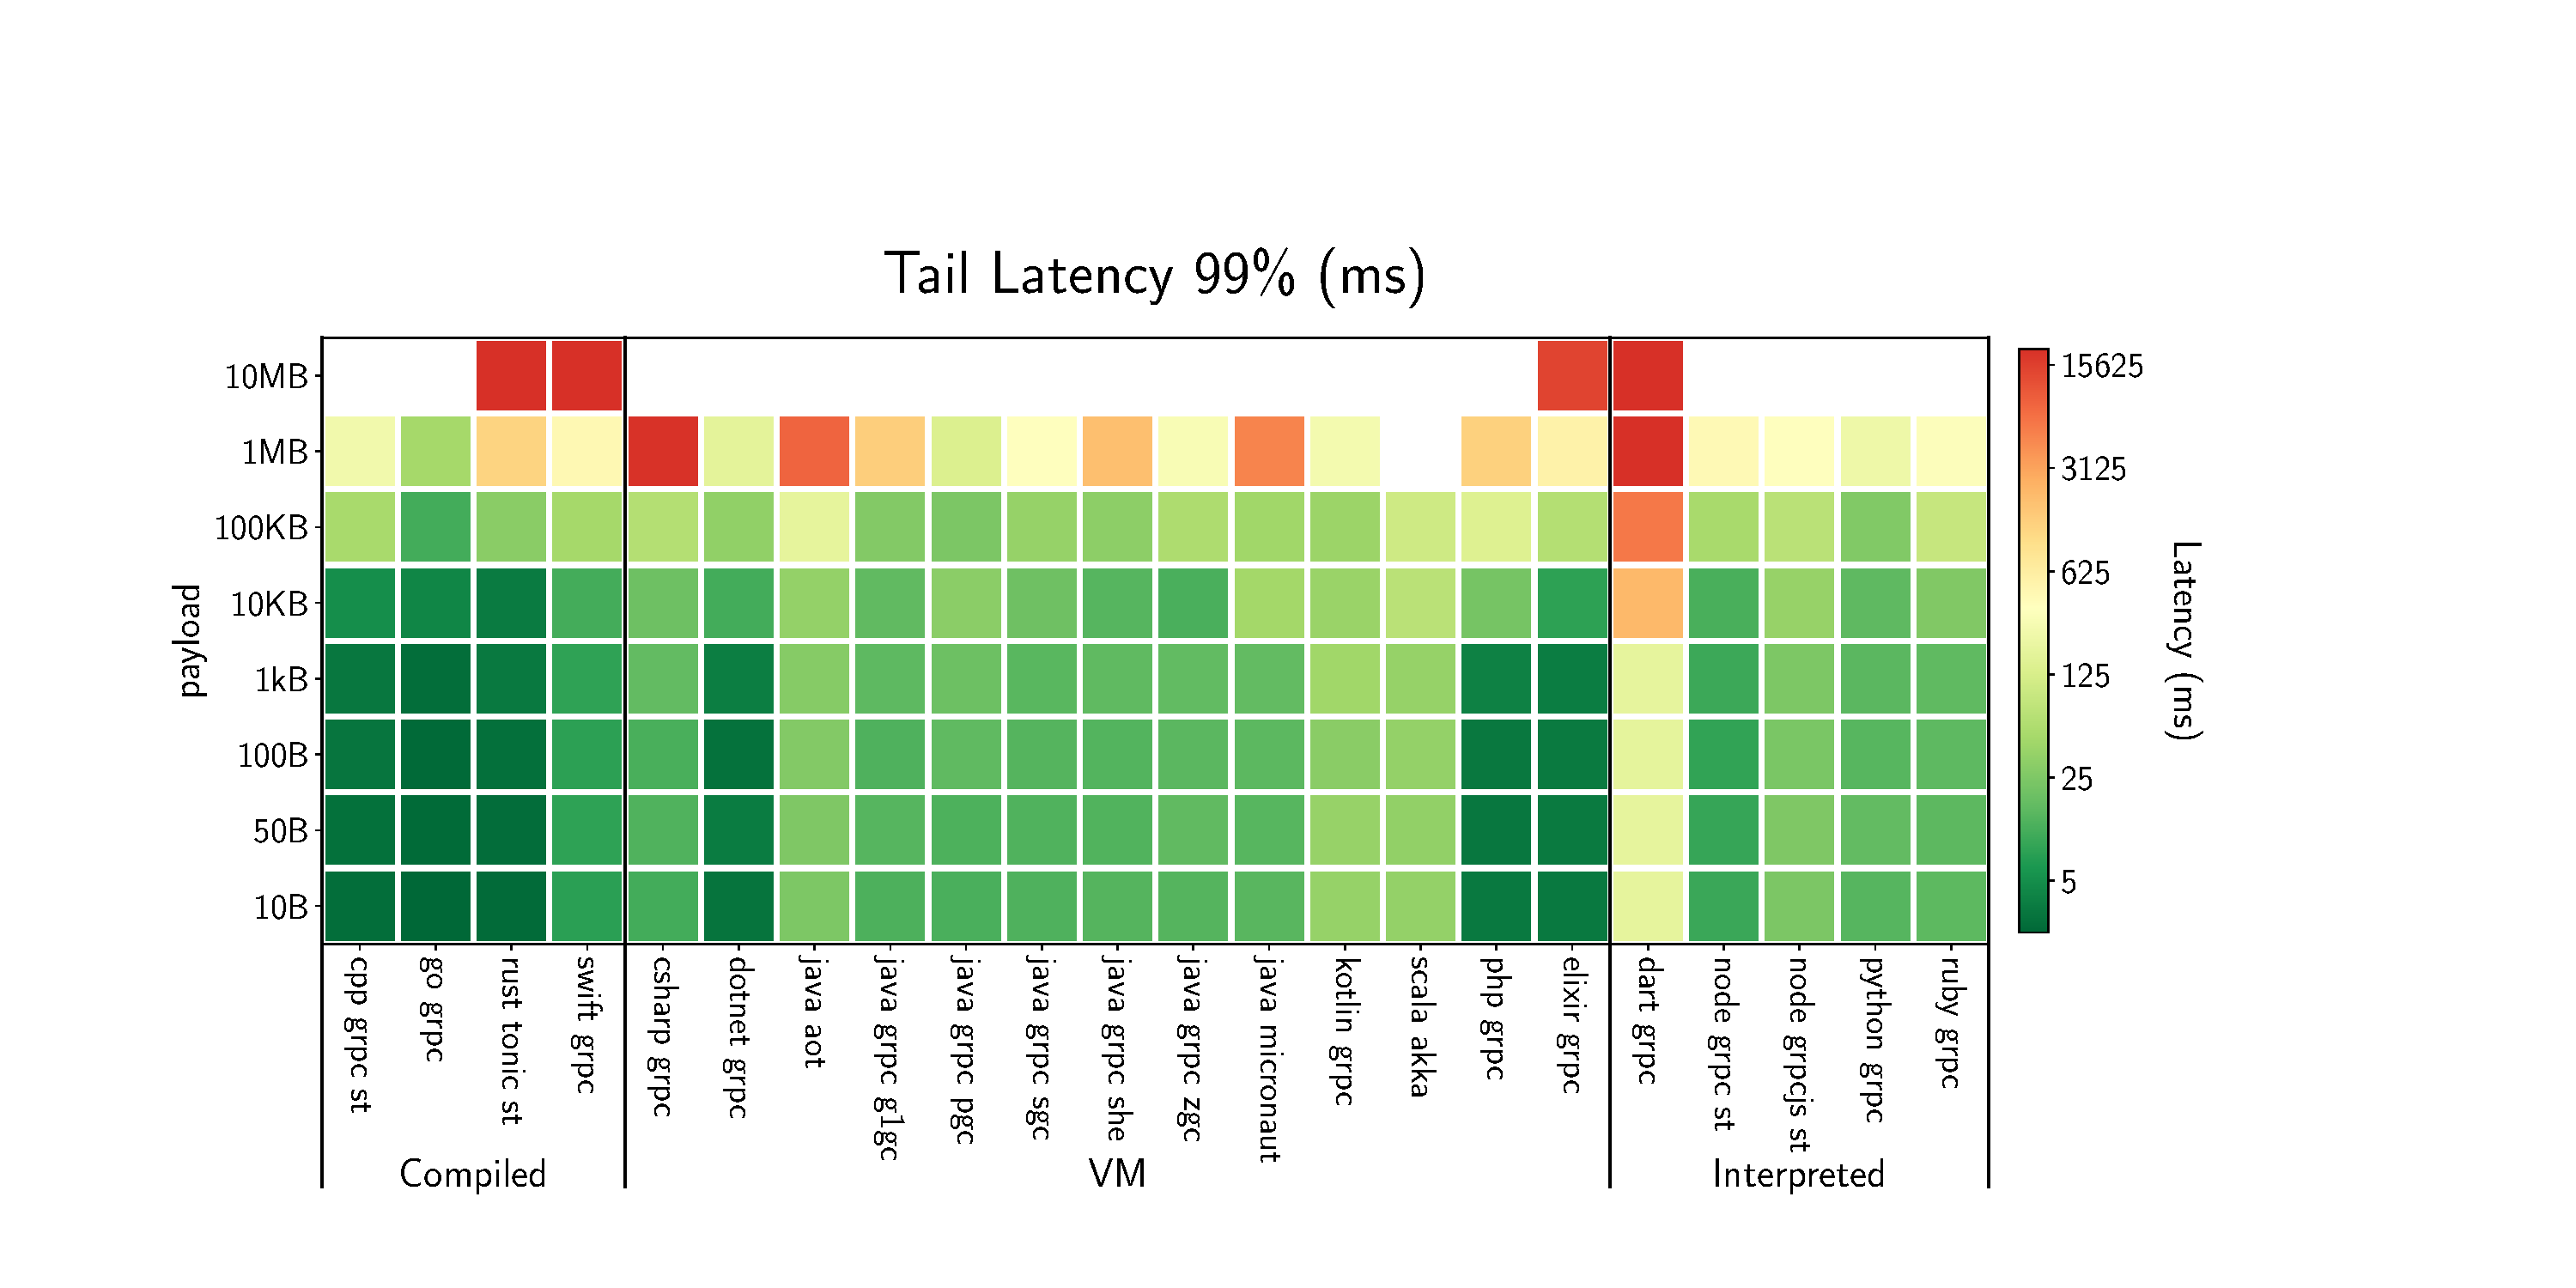
\includegraphics[width=1.2\linewidth]{imgs/rpc_images/tail99_payload}
    \end{center}
    \caption{Experemenal software architecture}\label{fig:tail99_payload}
\end{figure}


\subsection{Threads to validity}
\subsection{Conclusion}
